
%%%%%%%%%%%%%%%%%%%%%%% file typeinst.tex %%%%%%%%%%%%%%%%%%%%%%%%%
%
% This is the LaTeX source for the instructions to authors using
% the LaTeX document class 'llncs.cls' for contributions to
% the Lecture Notes in Computer Sciences series.
% http://www.springer.com/lncs       Springer Heidelberg 2006/05/04
%
% It may be used as a template for your own input - copy it
% to a new file with a new name and use it as the basis
% for your article.
%
% NB: the document class 'llncs' has its own and detailed documentation, see
% ftp://ftp.springer.de/data/pubftp/pub/tex/latex/llncs/latex2e/llncsdoc.pdf
%
%%%%%%%%%%%%%%%%%%%%%%%%%%%%%%%%%%%%%%%%%%%%%%%%%%%%%%%%%%%%%%%%%%%


\documentclass[runningheads]{llncs}
\usepackage{amsmath}
\usepackage{mathtools}
\usepackage{amssymb}
\usepackage{float}
\usepackage{multicol}

\setcounter{tocdepth}{3}
\usepackage{graphicx}
\usepackage[sorting=none]{biblatex}
\addbibresource{references.bib}



\usepackage{url}
\urldef{\mailsc}\path||    
\newcommand{\keywords}[1]{\par\addvspace\baselineskip
\noindent\keywordname\enspace\ignorespaces#1}

\begin{document}

\mainmatter  % start of an individual contribution

% first the title is needed
\title{Application of a chain-like and a hypercube communication topology 
in a multi-swarm PSO algorithm applied to continuous optimization problems}
% Los titulos no llevan punto al final - M

% a short form should be given in case it is too long for the running head
\titlerunning{José Guzmán, Mario Garcia}

% the name(s) of the author(s) follow(s) next
%
% NB: Chinese authors should write their first names(s) in front of
% their surnames. This ensures that the names appear correctly in
% the running heads and the author index.
%
\author{José Guzmán \and Mario García-Valdez}

\authorrunning{Guzmán et al.}
% (feature abused for this document to repeat the title also on left hand pages)

% the affiliations are given next; don't give your e-mail address
% unless you accept that it will be published
\institute{Tijuana Institute of Technology, Tijuana, Mexico
\email{jose.guzmanc19@tectijuana.edu.mx, mario@tectijuana.edu.mx}}



%
% NB: a more complex sample for affiliations and the mapping to the
% corresponding authors can be found in the file "llncs.dem"
% (search for the string "\mainmatter" where a contribution starts).
% "llncs.dem" accompanies the document class "llncs.cls".
%

\toctitle{}
\tocauthor{José Guzmán, Mario García-Valdez}

\maketitle


\begin{abstract}

In this paper, there will be a comparison of optimization politics regarding the
change in communication topologies in a multi-population PSO, witch are a variation of normal PSO that create various populations called swarms in order to improve certain aspects of the performance in the optimization, algorithm that is working in a new event-based architecture. The comparison has been done based on continuous optimization for benchmark functions and was between the original algorithm made into this new architecture called EvoSwarm and a variant of this witch has applied a chain topology and a hypercubic topology as communication policy. Showing that in the majority of the functions evaluated, the chain topology  ended up winning using the MSE as reference.

\keywords{PSO, EvoSwarm, multi-swarm intelligence, communication topologies,
 chain algorithm, hypercube, multi-swarm PSO.}
\end{abstract}


\section{Introduction}

Among the various strategies that have emerged in recent times for bio-inspired
optimization algorithms, the creation of multiple populations to work in
parallel and asynchronously has proven to be valuable \cite{a1}.
% Las citas se ponen antes del punto - M 
% Procurar no poner superlativos como 'the most'a menos que tengamos los datos - M 
One of the critical points in this technique is communication between populations, since it has been observed in various studies that the exchange of possible solutions helps to improve the performance of optimization algorithms \cite{a2}.
% Aquí falta un parrafo que conecte con lo que sigue, por ejemplo: 
Several distributed architectures have been proposed to manage the communication and parallel execution of these kind of algorithms, for example there is a similar approach by Scott Haberson et al using a multi-population parallel genetic algorithm for in depended evolution \cite{da1}.
% Aqui comenta algunos otros brevemente 
% con referencias - M 
% Conector: 
Recently, there is interest in cloud-native, event-based architectures suitable to run locally on a personal computer or in a cloud platform service. 
%% Ahora si: 
An event-based architecture uses events to trigger and communicate between services and processes. An event is a state change or an update, like an order placed in a food delivery application. Events can either carry the state (the item purchased, its price, and a delivery address) or be just identifiers (a notification that an order was shipped). Using an event-based architecture, we intend to carry out a series of experiments to analyze the effect of changing the communication topology in a multi-population optimization algorithm's performance. Using this type of architecture with a multi-swarm optimization algorithm is a new approach. There is an opportunity to find a substantial variation in the performance of such an optimization algorithm by changing the way the various swarms communicate to exchange information. 


In this paper, we concentrate our efforts on the specific case of using a chain and a hypercube topology in this new architecture. We chose these topologies for their ability to be adapted to the architecture mentioned above. They can work without altering the optimization algorithm allowing a fair comparison with other communication methods. In this work, we use only a PSO algorithm to assess the difference this simple change has on this algorithm.

This paper contains the following sections: The basic concepts used in this work are in Section 2. Section 3 contains the information regarding the proposed method. Section 4 presents experimental results, and in Section 5, the conclusions for this investigation.

\section{State of the Art}

% Tengo dudas de esta sección en un paper de congreso - M 
% Mejor poner aquí el State of the Art, los otros tipos de
% Multipoblación 
% Ya viendola bien, le podemos poner de nombre State of the Art 
% en lugar the basic concepts - M 

%\subsection{Swarm Intelligence}
“Swarm intelligence (SI) is the collective behavior of decentralized, self-organized, natural or artificial systems.” The concept is used in artificial intelligence work. The expression was first brought up by Gerardo Beni and Jing Wang in 1989 in the context of robotic cellular systems \cite{b4}. 

SI systems are mostly made of a population of simple particles that interact with each other and with their environment at a local level. The inspiration to make this kind of system comes from nature, especially biological systems. Particles follow very simple rules for their interactions and these interactions lead to the creation of a global "smart" behavior \cite{b5}.

%\subsection{PSO}
% Agregar un párrafo que conecte con esto:
Knowing that it is planned to work with different populations of swarms, the need to use an optimization algorithm that has an affinity with this technique and with swarm intelligence is generated. From what has been observed in countless works, some of them mentioned in this paper, PSO has great compatibility with the techniques that are intended to be used.

Particle Swarm Optimization (PSO) is an optimization algorithm inspired by some animals' behavior, such as flocks of birds or schools of fish. Since it was introduced in 1995 by  J. Kennedy and R. Eberhar, it has undergone several improvements.\cite{b1} % pon el nombre del autor - M -j
Since then, researchers have created different versions, which aimed at different
purposes, developed new applications in many areas, published theoretical
studies on the effects of various parameters, and proposed many many algorithm variants \cite{b2}. A basic version of the PSO algorithm works with a population (swarm) of possible solutions (particles). These particles move in the search space according to some simple formulas. The movements in the particles' search space are determined by their best-known position and by the best-known position of the entire swarm. As better positions are discovered, they will guide the swarm's movements. The process is repeated many times, so it is expected that a satisfactory solution will eventually be discovered, although this may not happen\cite{b3}.

\subsection{Multi-Swarm PSO}

Multi-swarm optimization is a variant of Particle Swarm Optimization (PSO) based  multiple swarms (or sub-swarm) instead of one. The basic flow in a multi-swarm optimization is that each sub-swarm focuses on a specific search space region. In contrast, a specific diversification method decides where and when to launch the sub-swarms. 

For example, Wave of Swarm of Particles \cite{b6}, this work bases its diversification technique on the "collision" of particles. When the particles close to each other, they are sent into new sub-swarms, preventing complete convergence. The Dynamic Multi-Swarm-Particle Swarm Optimizer\cite{b7} regroups the particles from the sub-swarms (if they have converged) into new sub-swarms periodically, so the new iteration of swarms are started with particles from the previous one. Locust swarms \cite{b8} are founded on a "devour and go" strategy after a sub-swarm "devours" a small fraction of the search space. In order to find a local optimum, explorers are deployed to search for new regions promising to "keep going."

In contrast to typical PSO swarms, sub-swarms are fed with some information about previous swarms. These could be the positions and velocities instead of having their initial parameters to be randomly selected. In general, the development of multi-swarm systems creates a new path of design decisions that did not exist during the original development of PSO. These design decisions have been have well-established guidelines thanks to the numerous studies on the topic, for example, the use of non-random initial positions and initial velocities leads to better re-sults in multi-swarm systems, which is not the case for individual swarms \cite{b9}.

Some of these decisions can be reached by relatively independent subcomponents that allow different optimization techniques to be tested. For example, the multi-swarm system UMDA-PSO \cite{b10} combines elements of particle swarm optimization, distribution estimation algorithm, and differential evolution in a multi-swarm hybrid method.



\subsection{Communication topologies in multi-swarm algorithms}

Multi-population-based methods have often been analyzed and used to improve the optimization performance of nature-inspired optimization algorithms. Researchers often divide the original population into small sub-populations for some purposes, for example, solving large-scale optimization problems and dynamic optimization problems. Existing studies on multi-population optimization show that it integrates easily into various nature-inspired optimization algorithms, and often performs better than using single-population optimization algorithms including global reference functions and real-world applications \cite{b11}\cite{b12}.

Other investigations, reviews, and surveys on multi-population methods have also been published in recent years, in which multi-population concepts are described using other terms like  'parallel,' 'Cooperative,' 'co-evolution,' and 'islands.' Its multi-threaded and parallel processing features that significantly speed up deployment time \cite{b13}\cite{b14}.

Based on the previous information, another problem is born, and it is how to handle communication between sub-populations. The following four parameters control communication between sub-populations: 
\begin{itemize}
    \item A communication speed that defines the number of solutions in a sub-population to share with other sub-populations.
    \item A communication policy that determines which solutions should be replaced by those of other sub-populations.
    \item A communication interval that establishes the frequency to execute the communication.
    \item A connection topology that defines how to connect sub-populations.

\end{itemize}

There have been some papers focused in optimizing the communication between swarms, for example the survey in reference \cite{b15} has a collection of different investigations around this subject. For example El-Abd and Kamel discussed the multiple factors that can change the behavior of multiple cooperating swarms, these factors included the communication strategy used and the number swarms. The experimental results demonstrated that a circular topology communication strategy has an overall better performance than those that simple share the global best of all the swarms\cite{b16}.
Another example and the source of inspiration for this paper, is one of Li and Zeng, who presented a multi-population agent based co-genetic algorithm with a chain-like structure for parallel global numerical optimization, where a close chain-like connection structure, a cycle chain-like connection structure and a dynamic neighborhood were used to improve the parallel optimization\cite{b17}.


\subsection{EvoSwarm}

EvoSwarm is a relatively new way of working with multi-populations algorithms, this method is based around a structure of queues that are ready to receive and send messages across a network of individual computers \cite{b18}. This structure behaves like a factory for optimization, allowing the user to optimize several populations simultaneously and allow different optimization algorithms. All of this while being a continuous optimizer means that any population in the process can re-enter the optimizing phase of the structure to be re-optimized. In Figure 1 it can be appreciated how the EvoSwarm communicates.

\begin{figure}[h]
\centering
\DeclareGraphicsExtensions{.jpg}
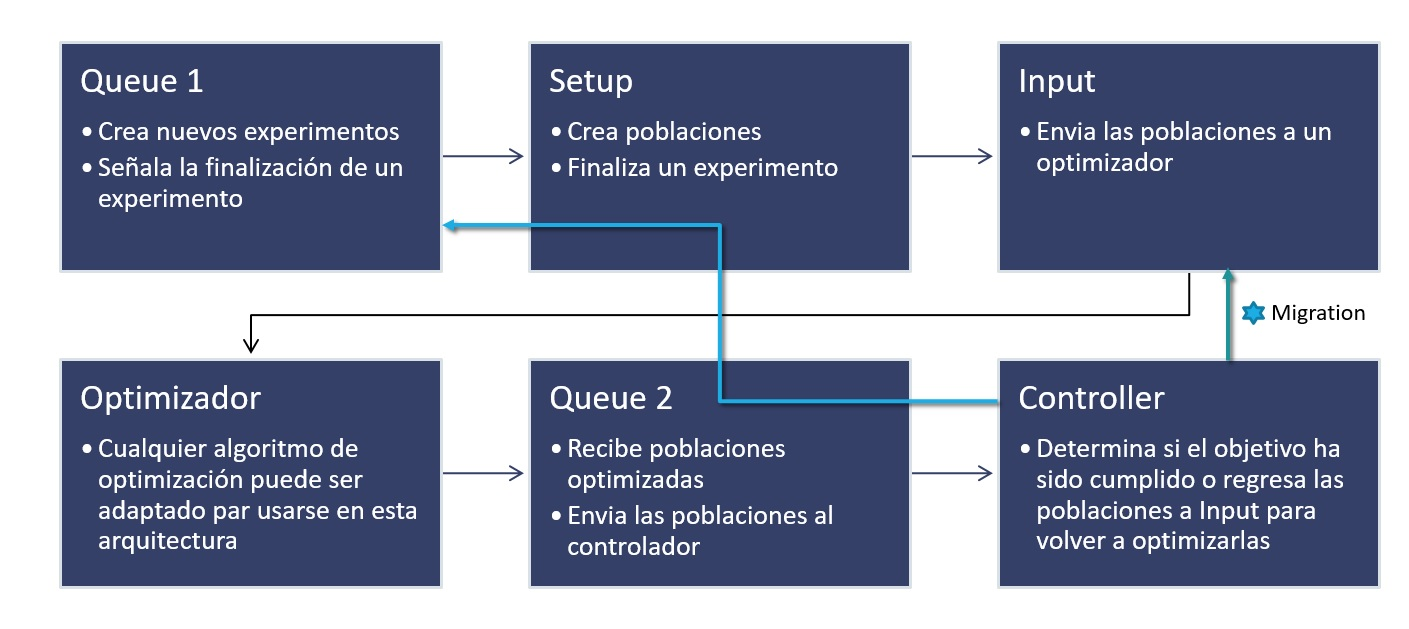
\includegraphics[scale=.40]{Resources/F1-1.jpg}
\caption{The EvoSwarm flow.}
\label{fig:example}
\end{figure}

It is worth mentioning that this architecture can be implemented using various computers in a network or using a virtualization tool, like in the case of this research using Docker. Here are some of the most important features that EvoSwarm brings to the user:

\begin{itemize}
    \item Fully capable of scalability, since more computers can be added to the network in order to manage a more significant workload.
    \item Independence between processes, which means that any process in the structure is completely separated from the other ones allowing more work to be done at the same time.
    \item It is adaptable to any population-based optimizing algorithm.
\end{itemize}


\section{Proposed method}

The proposed method consists of creating a variant of the architecture called EvoSwarm to observe any changes in performance. For this purpose, it is mandatory to be working with the same conditions as the original version. The only change made in this case was the communication policy between the populations of the multi-swarm PSO.

\subsection{PSO}
%Aqui mover a como esta en tesis
We implemented the software in Python; for the PSO algorithm, we use the Evolopy library \cite{b19}, as mention earlier in this paper, we use the same parameters for the PSO algorithm as the EvoSwarm paper (see Table 1).

\begin{table}[h!]
\centering
\caption{Parameters PSO of Evolopy libray}
\begin{tabular}{|c c|} 
 \hline
 Parameters & Values  \\ [0.5ex] 
 \hline\hline
 Vmax & 6 \\ 
 Wmax & 0.9 \\
 Wmin & 0.2 \\
C1 & 2 \\
C2 & 2 \\[0.5ex]
 \hline
\end{tabular}
\label{table:1}
\end{table}

\subsection{EvoSwarm}
Continuing with the configuration of the experiments, Table 2 presents the parameters used in EvoSwarm; these are for the 3 cases presented in this paper. 

\begin{table}[h]
\centering
\caption{Parameters for EvoSwarm}
\scalebox{0.90}{
\begin{tabular}{|c c c c c|} 
 \hline
 Dimensions & Generations  & Population size & Num. Experiments & Num. Population created\\ [0.2ex] 
 \hline\hline
 10 & 50 & 70 & 30 & 10 \\ 
 20 & 66 & 100 & 30 & 10 \\[0.2ex]
 \hline
\end{tabular}}
\label{table:1}
\end{table}

\subsection{Benchmark Functions}
%Aqui poner ref del pdf de coco
In order to run the optimization experiments, we selected ten functions from the COCO benchmark. We selected these functions because in our preliminary experiments, they showed performance variations as we changed the communication topology. Here are the ten functions:
\begin{multicols}{2}
\begin{itemize}

    \item Function 1: Sphere.
    \item Function 2: Elipsoid separable.
    \item Function 3: Rastrigin separable.
    \item Function 9: Rosenbrock rota-ted.
    \item Functions 10: Elipsoid.
    \item Function 15: Rastrigin.
    \item Function 17: Schaffer F7, condition 10.
    \item Function 18: Schaffer F7, condition 1000.
    \item Function 21: Gallagher 101 peaks.
    \item Function 22: Gallagher 21 peaks

\end{itemize}
\end{multicols}

The number given to each function comes from COCO. This means that any method using the benchmark can be compared against a great variety of optimization methods. The complete collection of functions, graphics, and equations can be reviewed in reference \cite{bbob}.

\subsection{EvoSwarm communication topology}
%diagrama maybe
In the original communication policy, the architecture waited until a minimum of three populations have reach the migration component, then these populations were sent into a process that combine the best half of each one the anothers. For example, let us name the three populations A, B, and C, then a sort method is applied to each one. The sorted populations now are divided into halves in preparation for the merging process, in with 3 “new” populations are born, the first one has the best half of A and B, the second has the best of B and C,and the third has the best of A and C. The last step is the reinsertion of these new populations into a queue in which they will be retaken by the PSO algorithm.

\subsection{Chain communication topology}
The first modification, in this case, is only to the merging process. To create a chained algorithm affect every three arriving populations will be sent into the migrations process, and like the original version, we sort the three populations. The modification consists in that the populations are only allowed to share a few members of the elite. In this case, 10. Individuals are carried into a chain structure in which a population can receive only one way of the structure and shares in another.

\begin{figure}
\centering
\DeclareGraphicsExtensions{.png,.pdf}
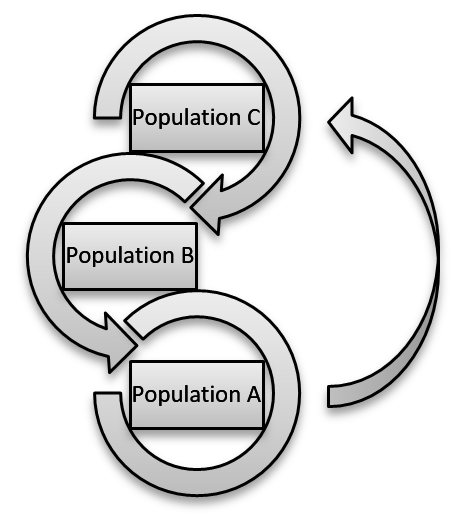
\includegraphics[width=0.35\linewidth]{Resources/F2.png}
\caption{Chain topology structure.}
\label{fig:example}
\end{figure}

\subsection{Hypercube communication topology}
The 2nd variation for the EvoSwarm structure is called a Hypercube; this one is based on a paper in which this topology was applied to solve a multi-reservoir of water using a multi-population algorithm \cite{b20}.  

This one is the most complicated topology presented in this paper. The name indicates this method has a cubic structure and can only be operated with eight populations at the same time or more. For this paper, we only need eight populations. Once the algorithm gets filled with eight populations, the migrations algorithm needs to assign each one a place in the hypercube structure. Figure 3 it has shown the layout of the structure.

\begin{figure}
\centering
\DeclareGraphicsExtensions{.png,.pdf}
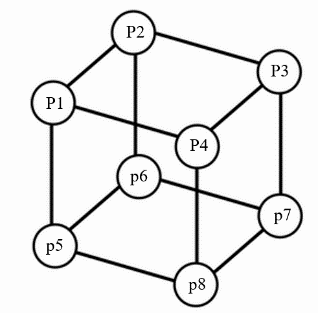
\includegraphics[width=0.35\linewidth]{Resources/F3.png}
\caption{Hypercube structure.}
\label{fig:example}
\end{figure}

The structure resembles a cube, and in every one of its vertices is one population. One thing that stands immediately is the capital P because only four populations have it, and was made this discrepancy between the two groups to represent a division. In this algorithm, we divided the Hypercube into two dimensions. Moreover, depending on the iteration of the experiment, the exchange of solutions is restricted.

Every iteration of an experiment changes the mode in which the populations communicate with each other. For example, in the first iteration, the eight populations can only communicate with the others in the same dimension. In the second iteration, the opposite happens, allowing them to exchange information with a population outside that dimension.   With eight vertices, only two exchanges are allowed, and for the experiments on this paper, only the best 10\% of solutions migrate to another swarm. 

\section{Experimental Results}
Table 3 shows the different MSE obtained in the experimentation.

\begin{table}[h]
    \centering
    \caption{Comparison of MSE obtained with the experiments, best results are in bold}
    \scalebox{0.72}{
    \begin{tabular}{|c|c||c|c|c||c|c|c|}
    \hline
     Dimensions & Function & EvoSwarm MSE & Chain MSE & Hypercube MSE & EvoSwarm Stdev & Chain Stdev & Hypercube Stdev \\ [0.5ex] 
    \hline\hline
    10 & 1	& \textbf{3.73447E-09} &	4.43163E-09 & 4.31567E-09 & 2.34E-09 & 2.68525E-09 & 3.10095E-09 \\ 
    10 & 2 & \textbf{3.78687E-09} & 4.88483E-09 & 3.95527E-09 & 2.84285E-09 & 2.46615E-09 & 2.95704E-09\\
    10 & 3 & 0.795723668 & \textbf{0.066330607} & 0.736180347 & 1.720290002 & 0.252429203 & 2.09770153 \\
    10 & 9 & 0.317521615 & \textbf{0.291698111} & 0.495606846 & 0.221999486 & 0.133724951 & 0.992888643 \\
    10 & 10 & 385.5382883 & \textbf{368.3836667} & 504.1392548 & 399.9278681 & 453.6655356 & 558.1741402 \\
    10 & 15 & 15.76249501 & \textbf{12.76554083} & 13.58271757 & 6.088547227 & 4.814606813 & 6.470316492 \\
    10 & 17 & \textbf{0.068348159} & 0.089892078 & 0.108848139 & 0.097958037 & 0.203665048 & 0.188877178 \\
    10 & 18 & 0.361780116 & \textbf{0.308286435} & 0.536340776 & 0.307789471 &0.364641853 & 0.53188395 \\
    10 & 21 & 0.241362711 & 0.330200323 & \textbf{0.129516888} & 0.518278881 & 0.588559758 & 0.343623139 \\
    10 & 22 & 0.58421438 & \textbf{0.337485965} & 0.947592035 & 0.698924145 & 0.614376298 & 1.092855278 \\
    20 & 1 & 5.5855E-09 & \textbf{5.29107E-09} & 5.60977E-09 & 2.54598E-09 & 3.08721E-09 & 2.78851E-09 \\
    20 & 2 & 0.70300253 & 2.214098553 & \textbf{5.51067E-09} & 3.850503404 & 12.12711719 & 2.43854E-09 \\
    20 & 3 & 8.506782382 & \textbf{6.523271752} & 6.566336254 & 7.91517587 & 6.962162793 & 6.445378042 \\
    20 & 9 & 11.75981164 & \textbf{11.28483752} & 11.54803115 & 1.257101321 & 1.070210208 & 1.150081504 \\
    20 & 10 & 5154.23155 & \textbf{4194.776213} & 4928.296717 & 4024.704045 & 3326.837717 & 4838.931553 \\
    20 & 15 & 57.76524461 & \textbf{55.55811032} & 58.12969092 & 16.78744293 & 17.2761844 & 13.78413645 \\
    20 & 17 & 0.807747361 & \textbf{0.65407833} & 0.87077806 & 0.377015722 & 0.323050832 & 0.450119262 \\
    20 & 18 & 2.648213694 & \textbf{2.136768786} & 2.51764207 & 1.402620032 & 0.898650887 & 1.195657371 \\
    20 & 21 & 0.624442455 & 0.2262255 & \textbf{0.2041556} & 0.903817073 & 0.486727692 & 0.513631785 \\
    20 & 22 & 2.030148903 & \textbf{1.578348414} & 1.915845972 & 1.821498605 & 1.638408845 & 1.869210661\\
    \hline
    \end{tabular}}
    \label{tab:my_label}
\end{table}
\hfill\break


\subsection{Statistical test}
We present the statistical tests below to compare the three methods applied in this work, comparing the two new methods with the original method and between them. In this case, we use a \(Z\) statistical test with an $\alpha$ of 0.5, giving a critical value to exceed 1.64; in Table 4, the comparison between the EvoSwarm method and the Chain method can be observed. Table 5 shows the comparison between EvoSwarm and the Hypercube method. Finally, Table 6 is the comparison between the methods and the Hypercube chain.\hfill \break
% Please add the following required packages to your document preamble:
% \usepackage{booktabs}
\begin{table}[H]
\caption{Statistical comparison for EvoSwarm vs Chain method, positive test results are in bold}
    \scalebox{0.99}{
\begin{tabular}{|c|c|c|c|c|c|}
\hline
Dimension & Function & EvoSwarm MSE & Chain MSE  & EvoSwarm vs Chain Z value & Z critic value \\
\hline
10        & 1        & 4.7861E-09   & 4.4579E-09 & 0.38385888                & 1.64           \\
10        & 2        & 3.8305E-09   & 4.1792E-09 & -0.51477671               & 1.64           \\
10        & 3        & 2.35292757   & 0.53764944 & \textbf{3.04132131}       & 1.64           \\
10        & 9        & 0.49249742   & 0.2527938  & 1.31849085                & 1.64           \\
10        & 10       & 250.173833   & 430.542073 & -1.71933543               & 1.64           \\
10        & 15       & 14.6650026   & 12.0546942 & \textbf{1.64153098}       & 1.64           \\
10        & 17       & 0.0923583    & 0.07576297 & 0.3984427                 & 1.64           \\
10        & 18       & 0.52485291   & 0.50641272 & 0.12824242                & 1.64           \\
10        & 21       & 0.32985228   & 0.23742293 & 0.64359863                & 1.64           \\
10        & 22       & 0.69206415   & 0.51478211 & 1.05251019                & 1.64           \\
20        & 1        & 0.03594249   & 5.5523E-09 & 0.99999998                & 1.64           \\
20        & 2        & 5.6467E-09   & 5.4975E-09 & 0.23720531                & 1.64           \\
20        & 3        & 12.082746    & 8.74663868 & 1.57882461                & 1.64           \\
20        & 9        & 11.1034972   & 11.370252  & -0.5302659                & 1.64           \\
20        & 10       & 4994.88899   & 4472.97104 & 0.55192392                & 1.64           \\
20        & 15       & 58.8810247   & 53.5457402 & 1.09914007                & 1.64           \\
20        & 17       & 0.78895834   & 0.76687862 & 0.19644001                & 1.64           \\
20        & 18       & 2.53338619   & 2.25526688 & 1.10707452                & 1.64           \\
20        & 21       & 0.90170655   & 0.39256696 & \textbf{2.09733952}       & 1.64           \\
20        & 22       & 3.6252321    & 1.51828786 & \textbf{2.6846472}        & 1.64         \\
\hline
\end{tabular}}
\end{table}
%EvoSwarm vs Hypercube
\begin{table}[H]
\caption{Statistical comparison for EvoSwarm vs Hypercube method, positive test results are in bold}
    \scalebox{0.90}{
\begin{tabular}{|c|c|c|c|c|c|}
\hline
Dimension & Function & EvoSwarm MSE & Hypercube MSE  & EvoSwarm vs Hypercube Z value & Z critic value \\
\hline
10 & 1  & 4.78611E-09 & 4.52861E-09 & 0.30205024  & 1.64 \\
10 & 2  & 3.83054E-09 & 4.65155E-09 & -1.19206785 & 1.64 \\
10 & 3  & 2.352927573 & 0.805637277 & \textbf{2.54675887}  & 1.64 \\
10 & 9  & 0.49249742  & 0.229809004 & 1.45323968  & 1.64 \\
10 & 10 & 250.1738327 & 374.4359744 & -1.71949324 & 1.64 \\
10 & 15 & 14.66500256 & 13.33777036 & 0.80707958  & 1.64 \\
10 & 17 & 0.0923583   & 0.087059177 & 0.12041284  & 1.64 \\
10 & 18 & 0.524852914 & 0.413659866 & 0.82306364  & 1.64 \\
10 & 21 & 0.329852279 & 0.20667313  & 0.91847447  & 1.64 \\
10 & 22 & 0.692064149 & 0.57179096  & 0.75725758  & 1.64 \\
20 & 1  & 0.03594249  & 5.54663E-09 & 0.99999998  & 1.64 \\
20 & 2  & 5.64673E-09 & 5.36566E-09 & 0.40712309  & 1.64 \\
20 & 3  & 12.082746   & 7.874205319 & \textbf{1.99114048}  & 1.64 \\
20 & 9  & 11.10349719 & 11.49485451 & -1.16267417 & 1.64 \\
20 & 10 & 4994.888993 & 5805.968994 & -0.60965616 & 1.64 \\
20 & 15 & 58.88102471 & 56.38870042 & 0.46747275  & 1.64 \\
20 & 17 & 0.788958338 & 0.764906251 & 0.20135086  & 1.64 \\
20 & 18 & 2.533386188 & 2.559019459 & -0.0776709  & 1.64 \\
20 & 21 & 0.901706552 & 0.395204608 & \textbf{2.23899811}  & 1.64 \\
20 & 22 & 3.625232097 & 1.650088133 & \textbf{2.59133147}  & 1.64 \\
\hline
\end{tabular}}
\end{table}

%Chain vs Hypercube

\begin{table}[H]
\caption{Statistical comparison for Chain vs Hypercube method, positive test results are in bold}
    \scalebox{0.99}{
\begin{tabular}{|c|c|c|c|c|c|}
\hline
Dimension & Function & Chain MSE & Hypercube MSE  & Chain vs Hypercube Z value & Z critic value \\
\hline
10 & 1  & 4.4579E-09 & 4.5286E-09 & -0.08393014 & 1.64 \\
10 & 2  & 4.1792E-09 & 4.6515E-09 & -0.62905414 & 1.64 \\
10 & 3  & 0.53764944 & 0.80563728 & -0.64672855 & 1.64 \\
10 & 9  & 0.2527938  & 0.229809   & 0.66826276  & 1.64 \\
10 & 10 & 430.542073 & 374.435974 & 0.49686142  & 1.64 \\
10 & 15 & 12.0546942 & 13.3377704 & -0.88253544 & 1.64 \\
10 & 17 & 0.07576297 & 0.08705918 & -0.26448643 & 1.64 \\
10 & 18 & 0.50641272 & 0.41365987 & 0.84096876  & 1.64 \\
10 & 21 & 0.23742293 & 0.20667313 & 0.27151497  & 1.64 \\
10 & 22 & 0.51478211 & 0.57179096 & -0.3220766  & 1.64 \\
20 & 1  & 5.5523E-09 & 5.5466E-09 & 0.00809714  & 1.64 \\
20 & 2  & 5.4975E-09 & 5.3657E-09 & 0.18397258  & 1.64 \\
20 & 3  & 8.74663868 & 7.87420532 & 0.43285509  & 1.64 \\
20 & 9  & 11.370252  & 11.4948545 & -0.26587439 & 1.64 \\
20 & 10 & 4472.97104 & 5805.96899 & -1.20027498 & 1.64 \\
20 & 15 & 53.5457402 & 56.3887004 & -0.57885803 & 1.64 \\
20 & 17 & 0.76687862 & 0.76490625 & 0.01653624  & 1.64 \\
20 & 18 & 2.25526688 & 2.55901946 & -0.94401758 & 1.64 \\
20 & 21 & 0.39256696 & 0.39520461 & -0.01355104 & 1.64 \\
20 & 22 & 1.51828786 & 1.65008813 & -0.34473831 & 1.64 \\
\hline
\end{tabular}}
\end{table}
\hfill
\break
\section{Conclusions}
In this research, we compared three communication methods between populations of a multi-swarm system to identify the variation in the result caused by these changes. However, the difference between most of the results is not very large. Nevertheless, there are scenarios in which the change was quite relevant, so it is possible to say that the change in communication policies significantly impacts multi-swarm methods for continuous optimization. In the same way, we must take into account that in this case, we only changed the type of communication between sub-swarms, which is only one of the policies that we can alter in this type of system. In future works, other policies can be altered at the same time to see what impact they will have. With the results obtained, we can infer that the change to the communication method is relevant for this type of system in specific situations. The alteration of the different work policies in multi-swarm systems could lead to greater specialization of these in specific scenarios.



\begin{thebibliography}{4}

\printbibliography


\end{thebibliography}


\end{document}
